% Describir el diseño o el planteamiento que ha sido utilizado para el desarrollo del componente, el cual depende del método seleccionado (hipotético-deductivo, inductivo, entre otros). Se sugiere incluir, los que correspondan:

% \begin{itemize}
%     \item Enfoque (cualitativo, cuantitativo o mixto).
%     \item Tipo de trabajo: exploratorio, descriptivo, explicativo, experimental, estudio de casos, entre otros.
%     \item Técnica de recolección de información (entrevistas, cuestionarios, análisis documental, entre otras).
%     \item Técnica de análisis de la información.
% \end{itemize}

% Este capítulo debe incluir toda la información necesaria para que un interesado pueda replicar el componente sin dificultades. Se debe mencionar explícitamente cuáles actividades se realizaron para cumplir con los objetivos planteados.

Para el desarrollo del proyecto se hizo uso de SCRUM \cite{SCRUM} como marco de trabajo a través de 4 sprints \cite{SCRUM-Sprints} (Tomando en cuenta el sprint 0). Cada subsección representa un Sprint en concreto. 

%%%%%%%%%%%%%%%%%%%%%%%%%%%%%%%%%%%%%%%%%%%
%--------------- SPRINT 0 ---------------%
%%%%%%%%%%%%%%%%%%%%%%%%%%%%%%%%%%%%%%%%%%%
\section{Sprint 0}
En este sprint denominado el \textit{"Sprint 0"}, se definieron aspectos fundamentales para el éxito del proyecto, con el objetivo de preparar al equipo y el entorno para los sprints de desarrollo regulares. 

\begin{itemize}
    \item Se realizó un análisis exhaustivo del stack tecnológico que se usará para el desarrollo, tanto del lado del frontend como del backend, abordando cada uno de los dos backends y los cuatro componentes diferentes del sistema, los cuales son:
    \begin{itemize}
        \item Gestión de perfiles de usuarios del sistema (Admin y pruebas de funcionalidad de usuarios logueados).
        \item Desarrollo de módulo que implemente funciones del tipo red social para los usuarios del sistema.
        \item Implementación de estrategia(s) de mediación o facilitación del consenso (sistema como mediador para el grupo de investigadores).
        \item Desarrollo del módulo de Analítica: Dashboards y estadísticas para la toma de decisiones.
    \end{itemize}
    El propósito de este análisis es garantizar que tanto el frontend como el backend utilicen las tecnologías más apropiadas para satisfacer los requisitos técnicos y de negocio, y para así asegurar una integración efectiva y eficiente entre todas las partes del sistema.
    

    Así se tomaron las siguientes decisiones:
    \begin{enumerate}
        \item Para la integración del sistema  en el lado del frontend se optó por utilizar Angular como framework de desarrollo, debido a que se puede reutilizar componentes de el sistema ResNet \cite{RESNET}. 
        \item Para el lado del backend se propuso utilizar Django como framework. Con Django, se espera aprovechar su robustez, seguridad y su capacidad para desarrollar rápidamente aplicaciones web escalables y de alto rendimiento. Además, Django ofrece una amplia gama de características integradas, como autenticación de usuarios, administración de bases de datos, y un ORM\footnote{ORM (Object-Relational Mapping) es una herramienta que facilita la comunicación y traducción de datos entre bases de datos relacionales y objetos en programación orientada a objetos.} potente, lo que lo hace una elección sólida para el desarrollo del backend del sistema. 
        \item Para mantener las mismas dependencias de desarrollo y simplificar la gestión del entorno, se utilizará Docker \cite{DOCKER}. Esto permite encapsular aplicaciones y sus dependencias en contenedores, asegurando consistencia entre entornos.
        \item Además, Docker Compose se empleará para orquestar el servidor backend y la base de datos, facilitando la configuración y gestión del entorno, y simplificando el despliegue del sistema en diferentes entornos.
        \item La elección de Neo4j se basa en la decisión de no alterar el modelo de datos actual. Dado que Neo4j está especialmente diseñado para modelos de datos conectados y relacionales, su adopción evita la necesidad de reestructurar el modelo existente, ahorrando tiempo y recursos mientras garantiza la continuidad del desarrollo del sistema.
        \item El control de versiones se hará mediante Git y para alojar dichas versiones se utilizará GitHub. Mediante una organización en donde se alojará el código fuente de los 4 componentes.
        \item Para la gestión del proyecto, se utilizó SCRUM en conjunto con Azure DevOps \cite{AZURE-DEVOPS}. SCRUM proporciona un marco ágil para la planificación y ejecución de proyectos, mientras que Azure DevOps \cite{AZURE-DEVOPS} ofrece herramientas integradas para facilitar todas las etapas del ciclo de vida del desarrollo de software. Esta combinación garantiza una gestión eficiente y colaborativa del proyecto, mejorando la transparencia y la entrega oportuna de resultados.
        En la Figura \ref{fig:azure-devops-project} se muestra el proyecto en Azure DevOps.
        \begin{figure}[H]
            \centering
            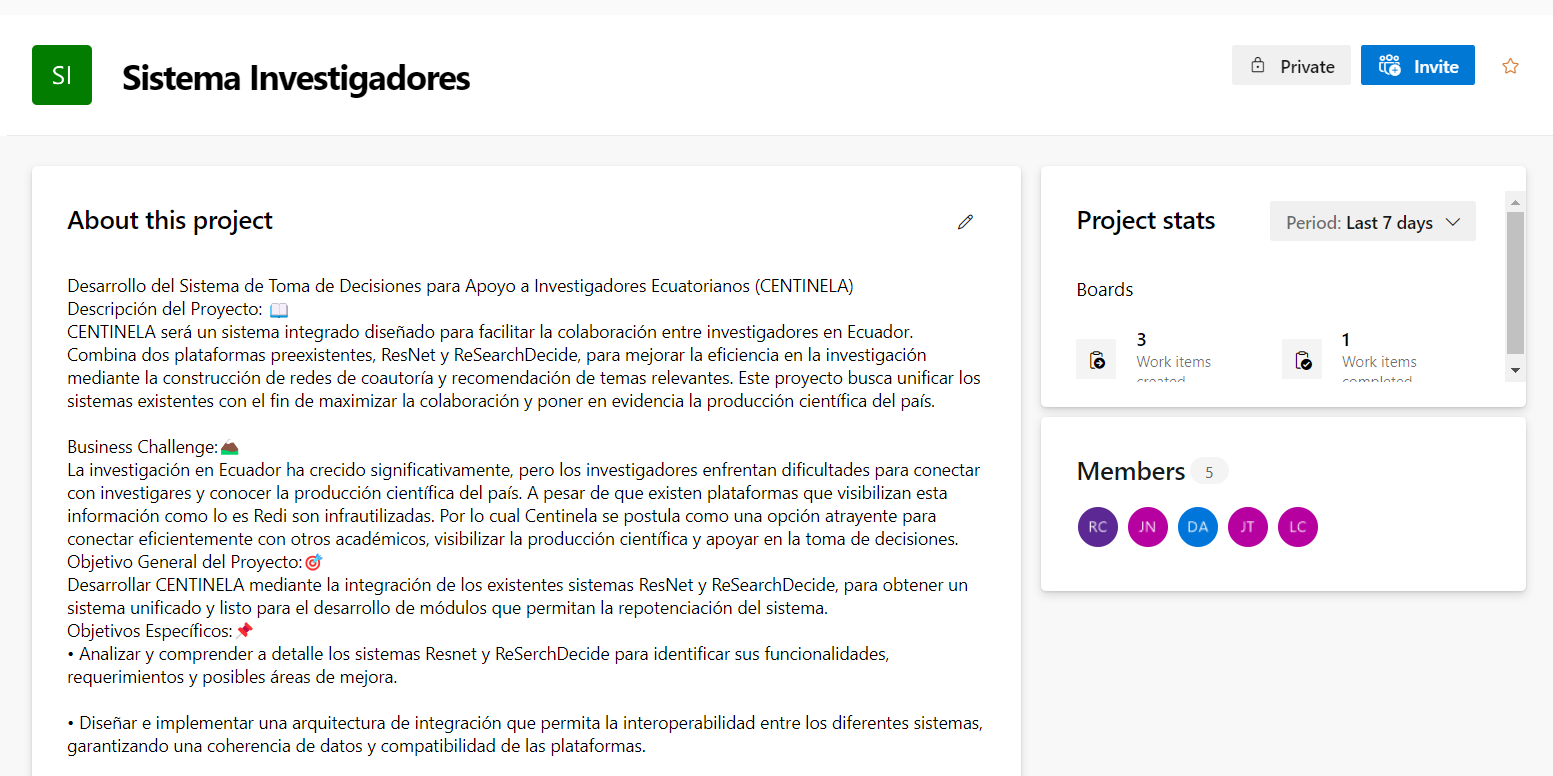
\includegraphics[width=0.5\linewidth]{../02Figures//02Chapter//Sprints//Sprint-0/azure-devops-project.png}
            \caption{Proyecto en Azure DevOps}
            \label{fig:azure-devops-project}
        \end{figure}
        \item Se optó por Visual Studio Code como editor de código para el frontend y PyCharm como IDE de desarrollo especializado para el backend. Esta elección proporcionó un entorno flexible y eficaz para la colaboración en el proyecto.
    \end{enumerate}

    \item Se establecieron horarios para las reuniones diarias, las cuales se llevarán a cabo los días lunes, martes, miércoles y jueves en el horario de 14:00 a 16:00 en un espacio proporcionado por la directora del proyecto, Lorena Recalde, en el edificio de Sistemas. Durante este intervalo, se realizaron los daily meetings y se llevó a cabo el trabajo en equipo.

    \item Se  decidió adoptar el inglés como el idioma oficial para la codificación, los commits y toda la documentación técnica dentro de nuestro equipo. Esta medida busca estandarizar nuestras prácticas con los estándares internacionales, facilitar la colaboración con otros equipos y mejorar la accesibilidad a recursos técnicos de alta calidad.

    \item Se decidió utilizar Arquitectura Hexagonal \cite{ARQUITECTURA-HEXAGONAL} como patrón de arquitectura, definiendo así una estructura de carpetas y respetando los principios de esta arquitectura. Cabe destacar que no se ha implementado arquitectura hexagonal en su totalidad, ya que se optó por una adaptación de la misma, obteniendo así una arquitectura de dos capas.
    \begin{itemize}
        \item \textbf{Backend}: Para el backend, en cuanto a  la estructura de carpetas, se definió que por cada módulo en general se tendrá las tres  capas de arquitectura como son infraestructura, aplicación y dominio como se muestra en la Figura \ref{fig:hexagonal-architecture-example-backend}.

        \begin{figure}[H]
            \centering
            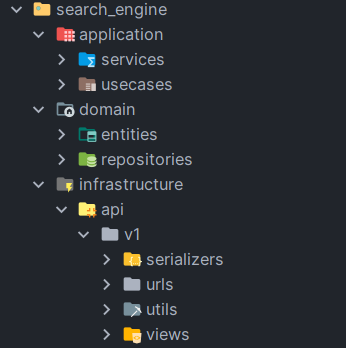
\includegraphics{../02Figures/02Chapter/Sprints/Sprint-0/hexagonal-architecture-example.png}
            \caption{Arquitectura Hexagonal aplicada en el modulo del motor de búsqueda}
            \label{fig:hexagonal-architecture-example-backend}
        \end{figure}
        \item \textbf{Frontend}: Basándonos en el concepto de puertos y adaptadores, en el frontend también hemos optado por  implementar la Arquitectura Hexagonal \cite{ARQUITECTURA-HEXAGONAL} como patrón de arquitectura, con algunas adaptaciones específicas para este contexto. Dado que el frontend se enfoca en la parte gráfica, el adaptador se denominará "presentación", donde se gestionará toda la interfaz gráfica. Esta capa de presentación será el punto de entrada hacia el núcleo (core) de la aplicación frontend, facilitando así una separación clara entre la lógica de negocio y la interfaz de usuario, y promoviendo una estructura modular y fácilmente mantenible (Figura \ref{fig:hexagonal-architecture-example-frontend}.)
        \begin{figure}[H]
            \centering
            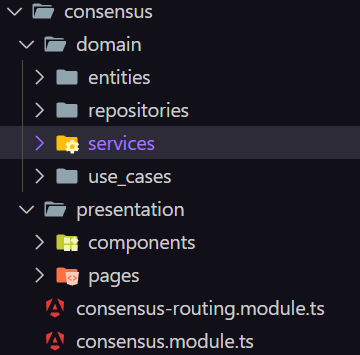
\includegraphics{../02Figures/02Chapter/Sprints/Sprint-0/hexagonal-architecture-example-frontend.png}
            \caption{Arquitectura hexagonal aplicada al modulo de consenso}
            \label{fig:hexagonal-architecture-example-frontend}
        \end{figure}
    \end{itemize}
\end{itemize}
%%%%%%%%%%%%%%%%%%%%%%%%%%%%%%%%%%%%%%%%%%%
%--------------- SPRINT 1 ---------------%
%%%%%%%%%%%%%%%%%%%%%%%%%%%%%%%%%%%%%%%%%%%
\section{Sprint 1}
\subsection{Introducción}
Durante este sprint, nuestro objetivo principal es crear diseños detallados que integren las funcionalidades de las aplicaciones Resnet (ver Sección \ref{chapter01-section03:ResNet}) y Research Decide en una plataforma unificada. Además, nos centraremos en identificar y proponer mejoras significativas para esta aplicación combinada. Utilizaremos Figma para desarrollar los mockups, aplicando los patrones de diseño más adecuados para asegurar una experiencia óptima para el usuario final. Es importante destacar que esta fase será iterativa, permitiendo ajustes y cambios continuos durante todo el desarrollo, por lo que la propuesta final no será definitiva.
\subsection{Objetivos del Sprint}

\begin{itemize}
    \item Diseñar el flujo de navegación de la aplicación combinada.
    \item Crear mockups de las interfaces de usuario de la aplicación.
    \item Desarrollar la estructura  principal del motor de búsqueda.
    \item Implementar el enrutamiento de la aplicación.
    \item Implementar la página de inicio de la aplicación.
\end{itemize}
\subsection{Planificación}
Para este sprint, hemos seleccionado las historias de usuario con su respectivo código enfocadas principalmente en la integración gráfica de las plataformas mencionadas en la Sección \ref{chapter01-section03:ResNet}, que se muestran en la Tabla \ref{C2T1:Historias de Usuario del Sprint 1}. 
Se debe tomar en cuenta que esta parte del desarrollo se enfoca en los usuarios que no necesariamente están registrados en la plataforma, por lo que se ha priorizado la visualización de información relevante para estos usuarios.
\begin{table}[H]
    \centering
    \begin{tabular}{|m{2.5cm}|m{5cm}|m{6cm}|}
        \hline
        \textbf{Identificador} &  \textbf{Historia de Usuario} & \textbf{Tareas} \\
        
        \hline
        Visual Studio Code & Como usuario no registrado deseo poder encontrar artículos relevantes dado un  tema de investigación para poder acceder rápidamente a información útil y actualizada que apoye mi estudio o trabajo  &  
        \begin{itemize}
            \item Componente para listar \break artículos
            \item Paginación para extraer resultados limitados
            \item Componente para filtrar la información por años
            \item Enrutamiento para redirigir hacia la página del articulo
            \item Página para visualizar información general del articulo
            
        \end{itemize} 
        \\
        \hline
          Visual Studio Code & Como usuario no registrado deseo poder ver los investigadores que tengan colaboraciones en artículos con afiliaciones ecuatorianas para mantenerme informado sobre sus investigaciones y campos de estudio &  
        \begin{itemize}
            \item Componente para listar Artículos
            \item Paginación para extraer resultados limitados
            \item Componente para filtrar la información por años
            \item Enrutamiento para redirigir hacia  la página del Articulo
            \item Página para visualizar información general del Articulo
            
        \end{itemize} 
        \\
        \hline
        
    \end{tabular}
    \caption{Historias de Usuario del sprint 1}
    \label{C2T1:Historias de Usuario del Sprint 1}
\end{table}


Todas las historias de usuario se han dividido en tareas más pequeñas y manejables. 
También en las Figuras \ref{fig:aceptance-criteria-HU-SE-01}  y  \ref{fig:aceptance-criteria-HU-SE-02} se muestran los criterios de aceptación de cada historia de usuario, que se utilizarán para verificar si la historia de usuario se ha completado correctamente.
\begin{figure}[H]
    \centering
    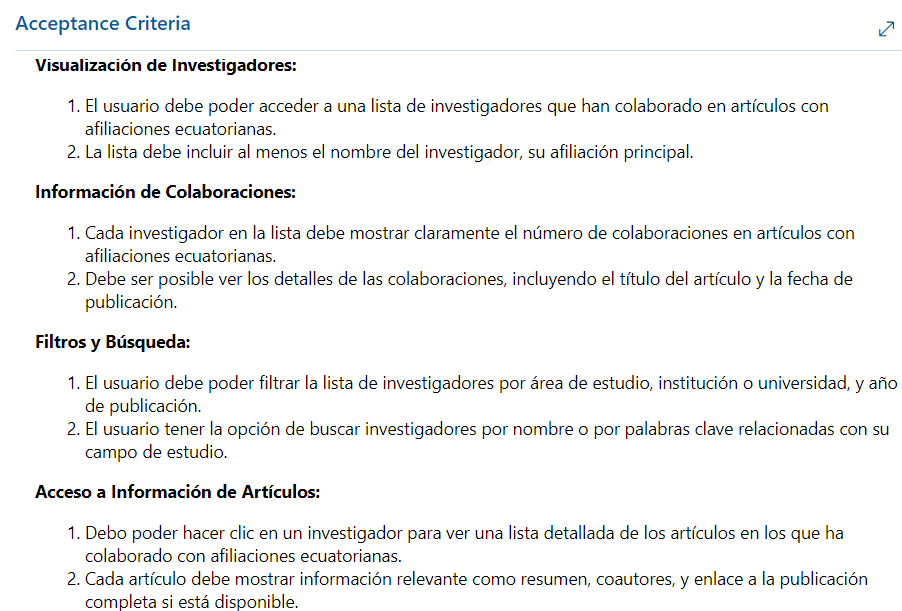
\includegraphics[scale=0.7]{../02Figures/02Chapter/Sprints/Sprint-1/aceptance-criteria-HU-SE-01.png}
    \caption{Criterios de aceptación de la historia de usuario HU-SE-01}
    \label{fig:aceptance-criteria-HU-SE-01}
\end{figure}
\begin{figure}[H]
    \centering
    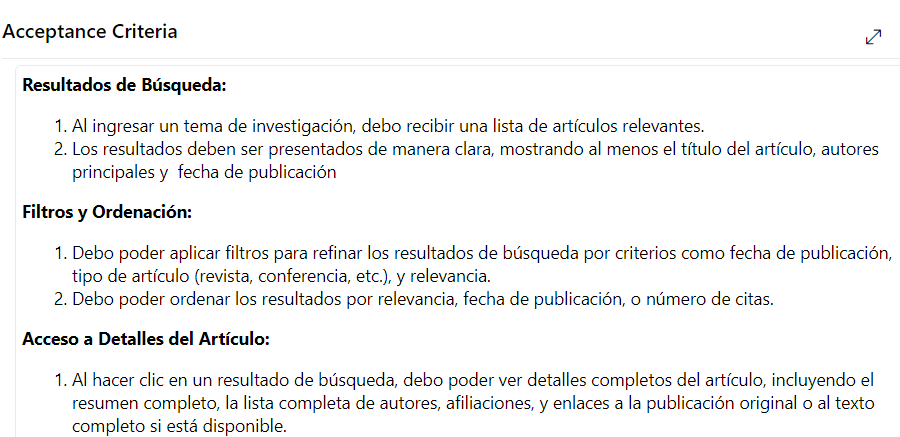
\includegraphics[scale=0.7]{../02Figures/02Chapter/Sprints/Sprint-1/aceptance-criteria-HU-SE-02.png}
    \caption{Criterios de aceptación de la historia de usuario HU-SE-02}
    \label{fig:aceptance-criteria-HU-SE-02}
\end{figure}


Estas historias de usuario se han priorizado en función de su importancia y complejidad, y se han asignado a los miembros del equipo de desarrollo. La Figura \ref{fig:azure-board-sprint-1} muestra las tareas asignadas a cada miembro del equipo.
\begin{figure}[H]
    \centering
    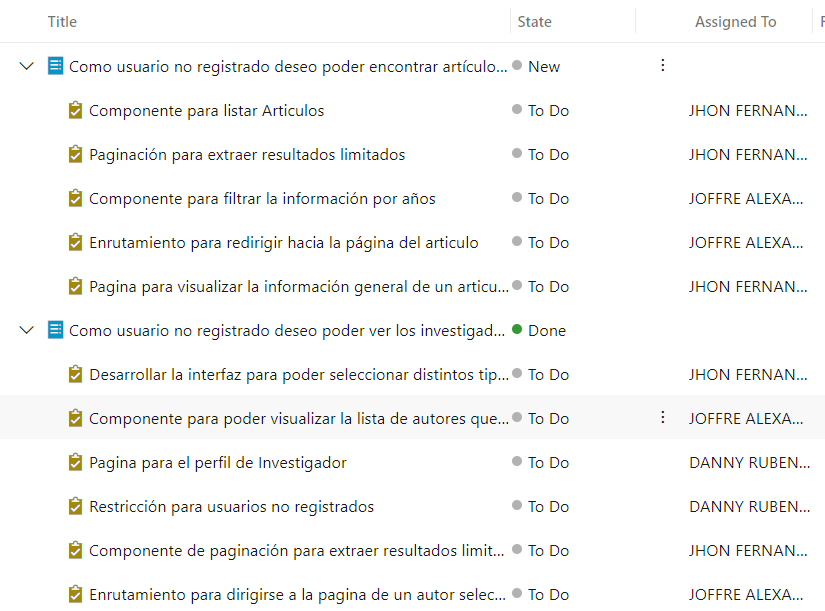
\includegraphics[scale=0.9]{../02Figures/02Chapter/Sprints/Sprint-1/fig_azure-board-sprint-1.png}
    \caption{Planificación de tareas del Sprint 1}
    \label{fig:azure-board-sprint-1}
\end{figure}

\subsection{Implementación}
Para la implementación de las historias de usuario, se ha utilizado la herramienta de diseño Figma, que permite crear prototipos de alta y baja fidelidad. 
A continuación, se presentan los mockups de las interfaces de usuario de la aplicación que se han desarrollado durante este sprint.
Cabe destacar que se siguió un proceso iterativo, por lo que los mockups presentados no son definitivos y pueden sufrir cambios en futuras iteraciones.
Además el diseño se baso en el patrón de diseño Mobile First \cite{MOBILE-FIRST}, que consiste en diseñar primero la versión móvil de la aplicación y luego adaptarla a dispositivos de mayor tamaño.

\subsubsection{Página de inicio}
La página de inicio de la aplicación es la primera pantalla que verá el usuario al ingresar a la plataforma. 
En esta pantalla, se mostrarán las opciones de búsqueda y un conjunto de datos sobre la información que tiene Centinela. Así como también una barra de navegación que permitirá al usuario acceder a otras secciones de la aplicación. 
La figura \ref{fig:mockup-home} muestra el diseño de la página de inicio.

\begin{figure}[H]
    \centering
    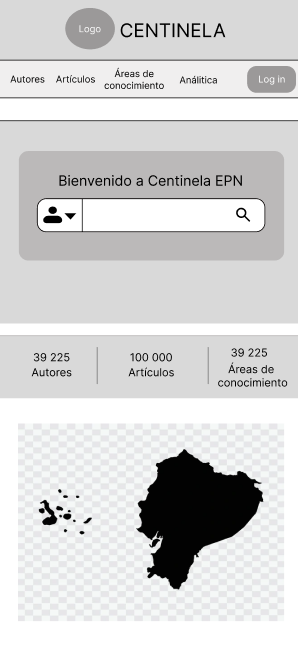
\includegraphics[scale=0.9]{../02Figures/02Chapter/Sprints/Sprint-1/mobile-first-home.png}
    \caption{Mockup de la página de inicio}
    \label{fig:mockup-home}
\end{figure}

Como se menciono en la sección \ref{chapter02-section02-sprint0} se utilizara una adaptación de arquitectura hexagonal para desarrollar la estructura de la aplicación.
Dando como resultado la estructura de carpetas que se muestra en la figura \ref{fig:hexagonal-architecture-home}.
Puesto que la página de inicio es la primera pantalla que verá el usuario al ingresar a la plataforma, se ha decidido crear una carpeta específica para esta sección.
También debido a que angular es un framework que se maneja con componentes, se ha creado un componente para la página de inicio, el cual se encuentra en la carpeta de pages.
A su vez  se ha creado el archivo de tipo module para la página de inicio, el mismo nos permitirá importar los componentes necesarios para la página de inicio, sin tener que importarlos en el archivo principal de la aplicación.
Este enfoque permitirá que el modulo de la página de inicio sea independiente del resto de la aplicación, que juntado con la arquitectura hexagonal facilitara la escalabilidad y mantenimiento de la aplicación.

\begin{figure}[H]
    \centering
    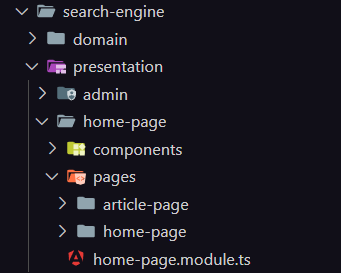
\includegraphics[scale=0.8]{../02Figures/02Chapter/Sprints/Sprint-1/home-page-ha.png}
    \caption{Estructura de carpetas de la página de inicio}
    \label{fig:hexagonal-architecture-home}
\end{figure}

Resultado de la implementación de la página de inicio se muestra en la figura \ref{fig:home-page}.
En la que se muestra la barra de navegación, el formulario de búsqueda y la información que tiene Centinela. El formulario de búsqueda cuenta con 3 opciones, 
la primera es para buscar por palabra clave a un autor, la segunda es para buscar autores relevantes dado un tópico de investigación y la tercera es para buscar artículos relevantes dado un tópico.
Bajo el motor de búsqueda se muestra el resumen del numero de artículos, autores y tópicos que tiene registrado Centinela.
Finalmente contiene un mapa que mostrará en que el número de artículos que se han publicado en cada provincia del Ecuador.
\begin{figure}[H]
    \centering
    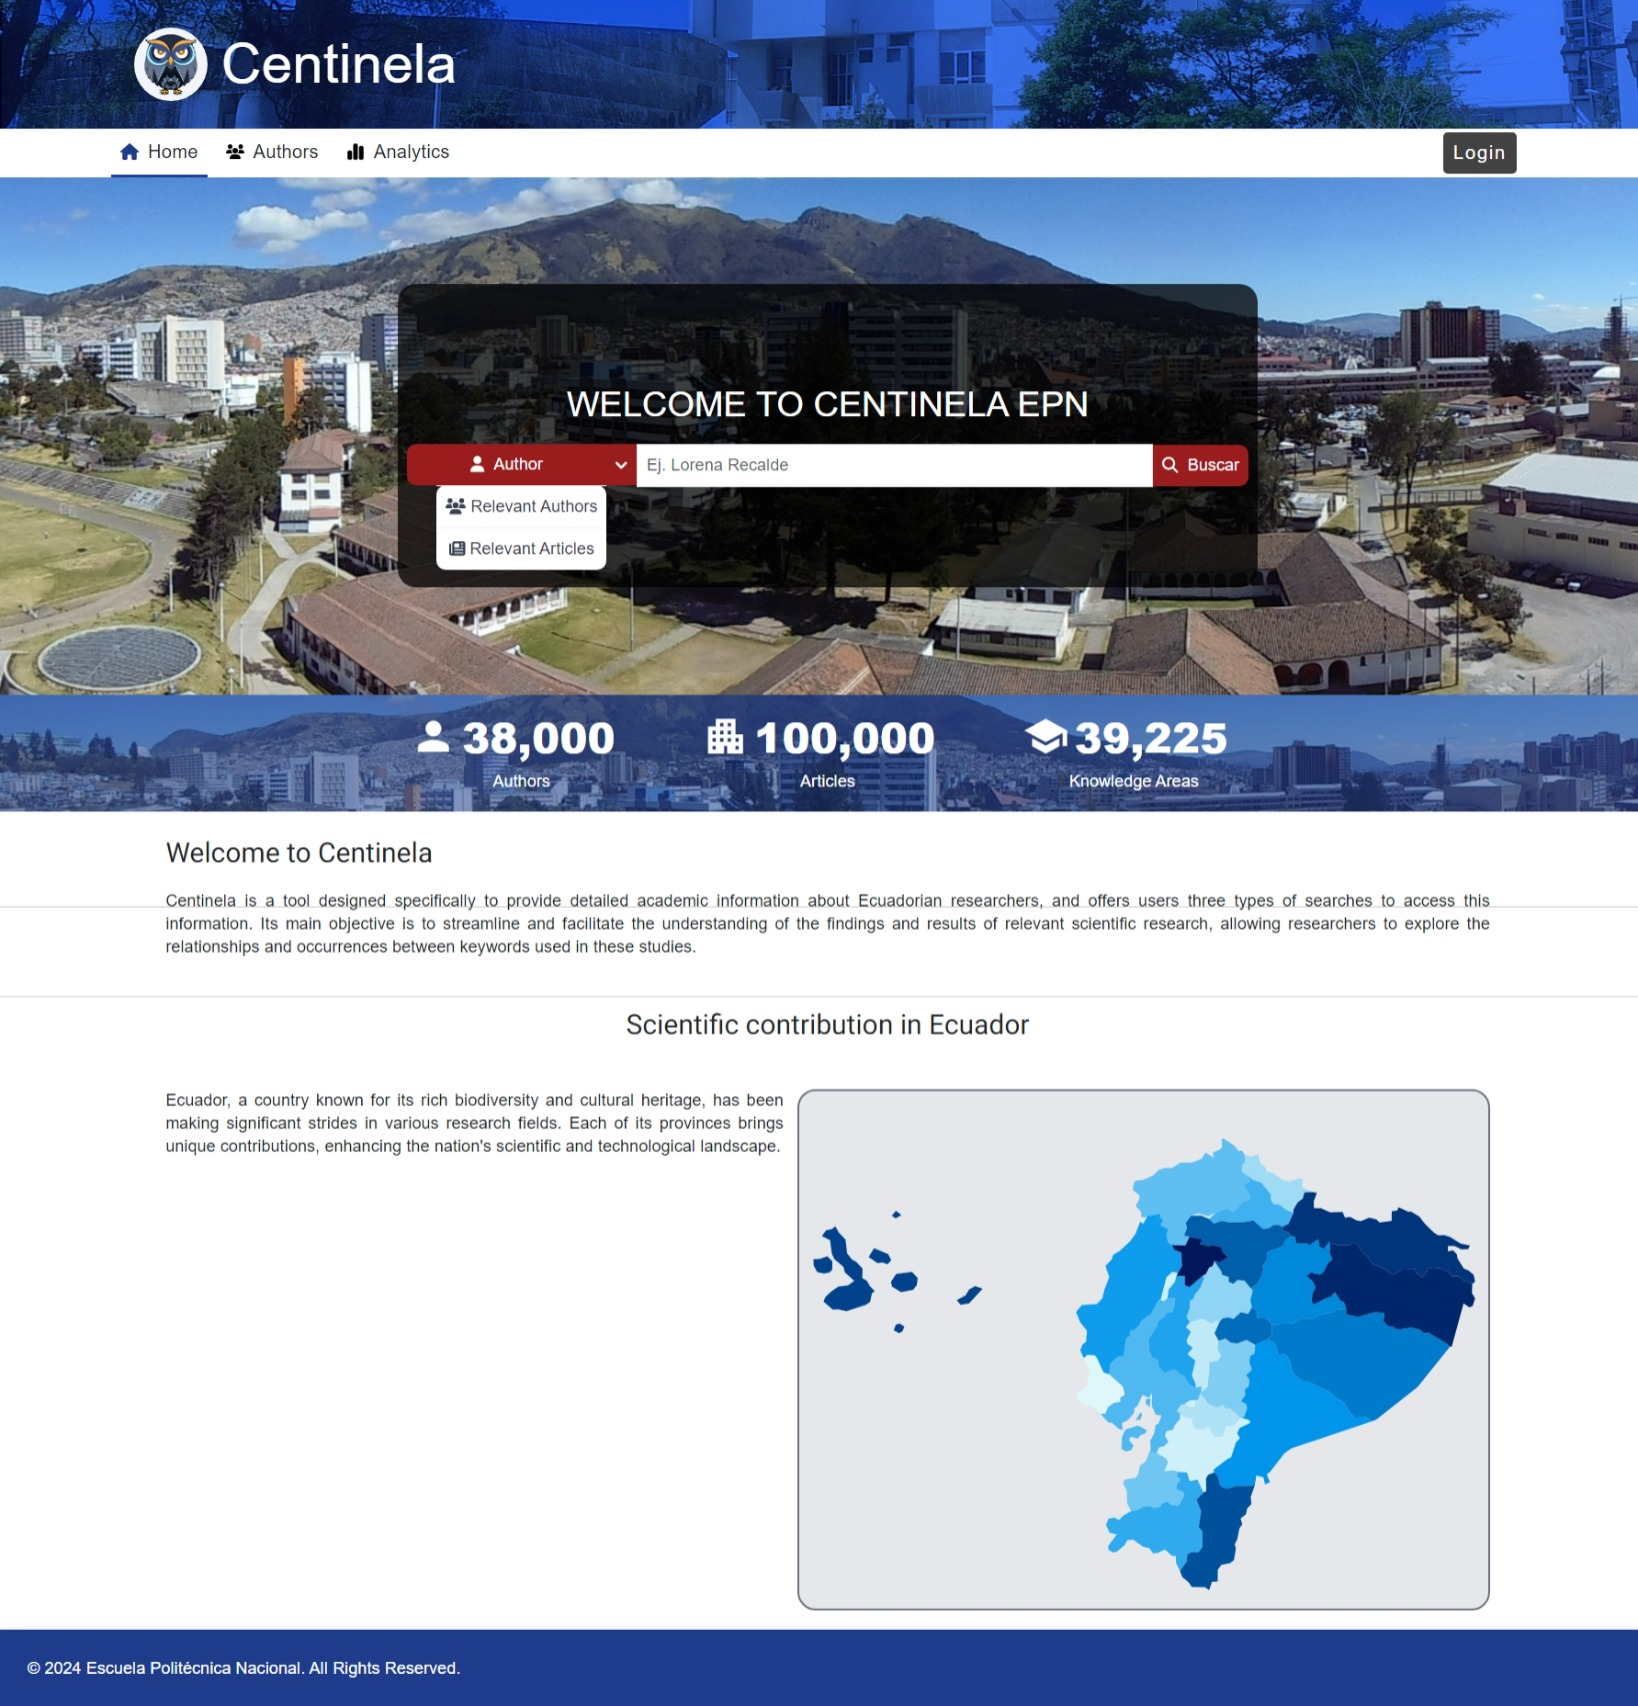
\includegraphics[scale=0.160]{../02Figures/02Chapter/Sprints/Sprint-1/home-page.jpeg}
    \caption{Página de inicio}
    \label{fig:home-page}
\end{figure}

\subsubsection{Página de resultados}
La página de resultados es la pantalla que se mostrará al usuario después de realizar una búsqueda en la aplicación.
En esta pantalla, se mostrarán los resultados de la búsqueda, que incluirán una lista de autores y artículos relevantes, dependiendo del tipo de búsqueda que haya realizado el usuario.
La figura \ref{fig:mockup-results} muestra el diseño de la página de resultados. Cabe destacar que esta página va a ser dinámica, es decir se modificará en función de los resultados de la búsqueda.
También contiene el componente de paginación, que permitirá al usuario navegar entre los resultados de la búsqueda. Este último está disponible para el tipo de búsqueda de autores por palabra clave y para el tipo de búsqueda de artículos relevantes por tópico, ya que estos tipos de búsqueda pueden devolver un gran número de resultados. Y al ser una aplicación web, se ha optado por mostrar 10 resultados por página para garantizar una buena experiencia de usuario y reducir tiempos de carga.

\begin{figure}[H]
    \centering
    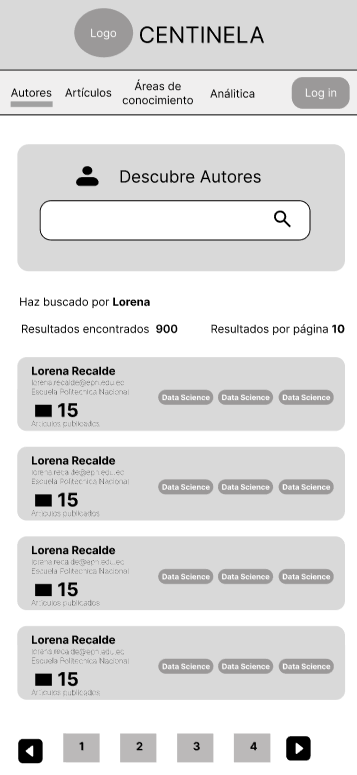
\includegraphics[scale=0.6]{../02Figures/02Chapter/Sprints/Sprint-1/mobile-first-results.png}
    \caption{Mockup de la página de resultados}
    \label{fig:mockup-results}
\end{figure}

Como se menciono en la Tabla \ref{fig:aceptance-criteria-HU-SE-01} y \ref{fig:aceptance-criteria-HU-SE-02} los criterios de aceptación de las historias de usuario HU-SE-01 y HU-SE-02 cada resultado tendrá que ser redirigido a una pantalla en donde 
se visualizará la información detallada del autor o del articulo. Para este caso en especifico se muestra el diseño para la pagina que tendrá
la información detallada de un autor, en la figura \ref{fig:mockup-article-detail}.
\begin{figure}[H]
    \centering
    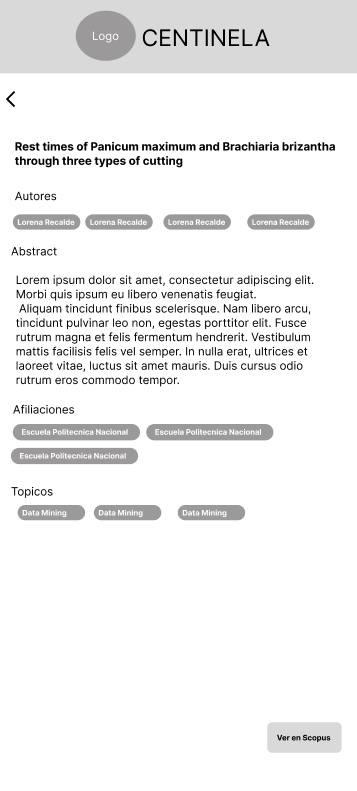
\includegraphics[scale=0.8]{../02Figures/02Chapter/Sprints/Sprint-1/article-detail.png}
    \caption{Mockup de la página de detalle del articulo}
    \label{fig:mockup-article-detail}
\end{figure}

Para el enrutamiento de la aplicación se ha utilizado el modulo de enrutamiento de Angular, el cual nos permite definir las rutas de la aplicación y asociarlas con los componentes correspondientes.
En la Figura \ref{fig:enrutamiento-article-page} se muestra el enrutamiento hacia el componente que contendrá la información general de un articulo. El mismo que como parámetro recibirá el id del articulo que se desea visualizar.
\begin{figure}[H]
    \centering
    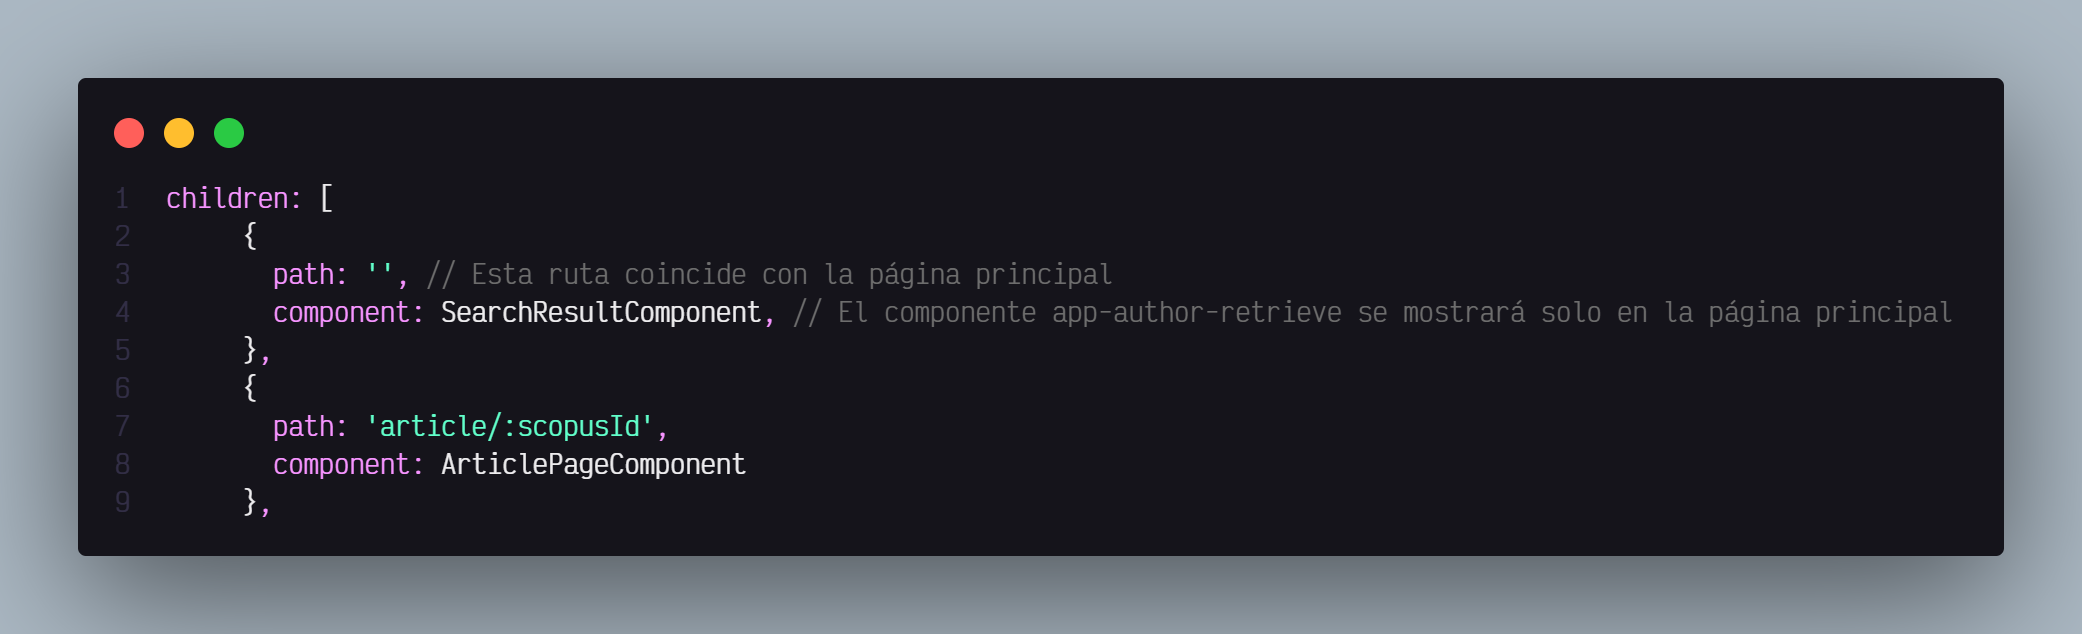
\includegraphics[scale=0.2]{../02Figures/02Chapter/Sprints/Sprint-1/enrutamiento-article-page.png}
    \caption{Routing de la página de detalle de articulo}
    \label{fig:enrutamiento-article-page}
\end{figure}

%% Aqui deseo mostrar ya la implementacion de la pagina de articulo pero da una descripcion de la misma
Resultado de la implementación de la página de información general de un articulo se muestra en la figura \ref{fig:article-page}.
En la que se muestra la información general de un articulo, como el titulo, resumen, autores, afiliaciones, palabras clave y el año de publicación. Asi como tambien un boton que permitira al usuario acceder al articulo completo en la pagina de Scopus.

\begin{figure}[H]
    \centering
    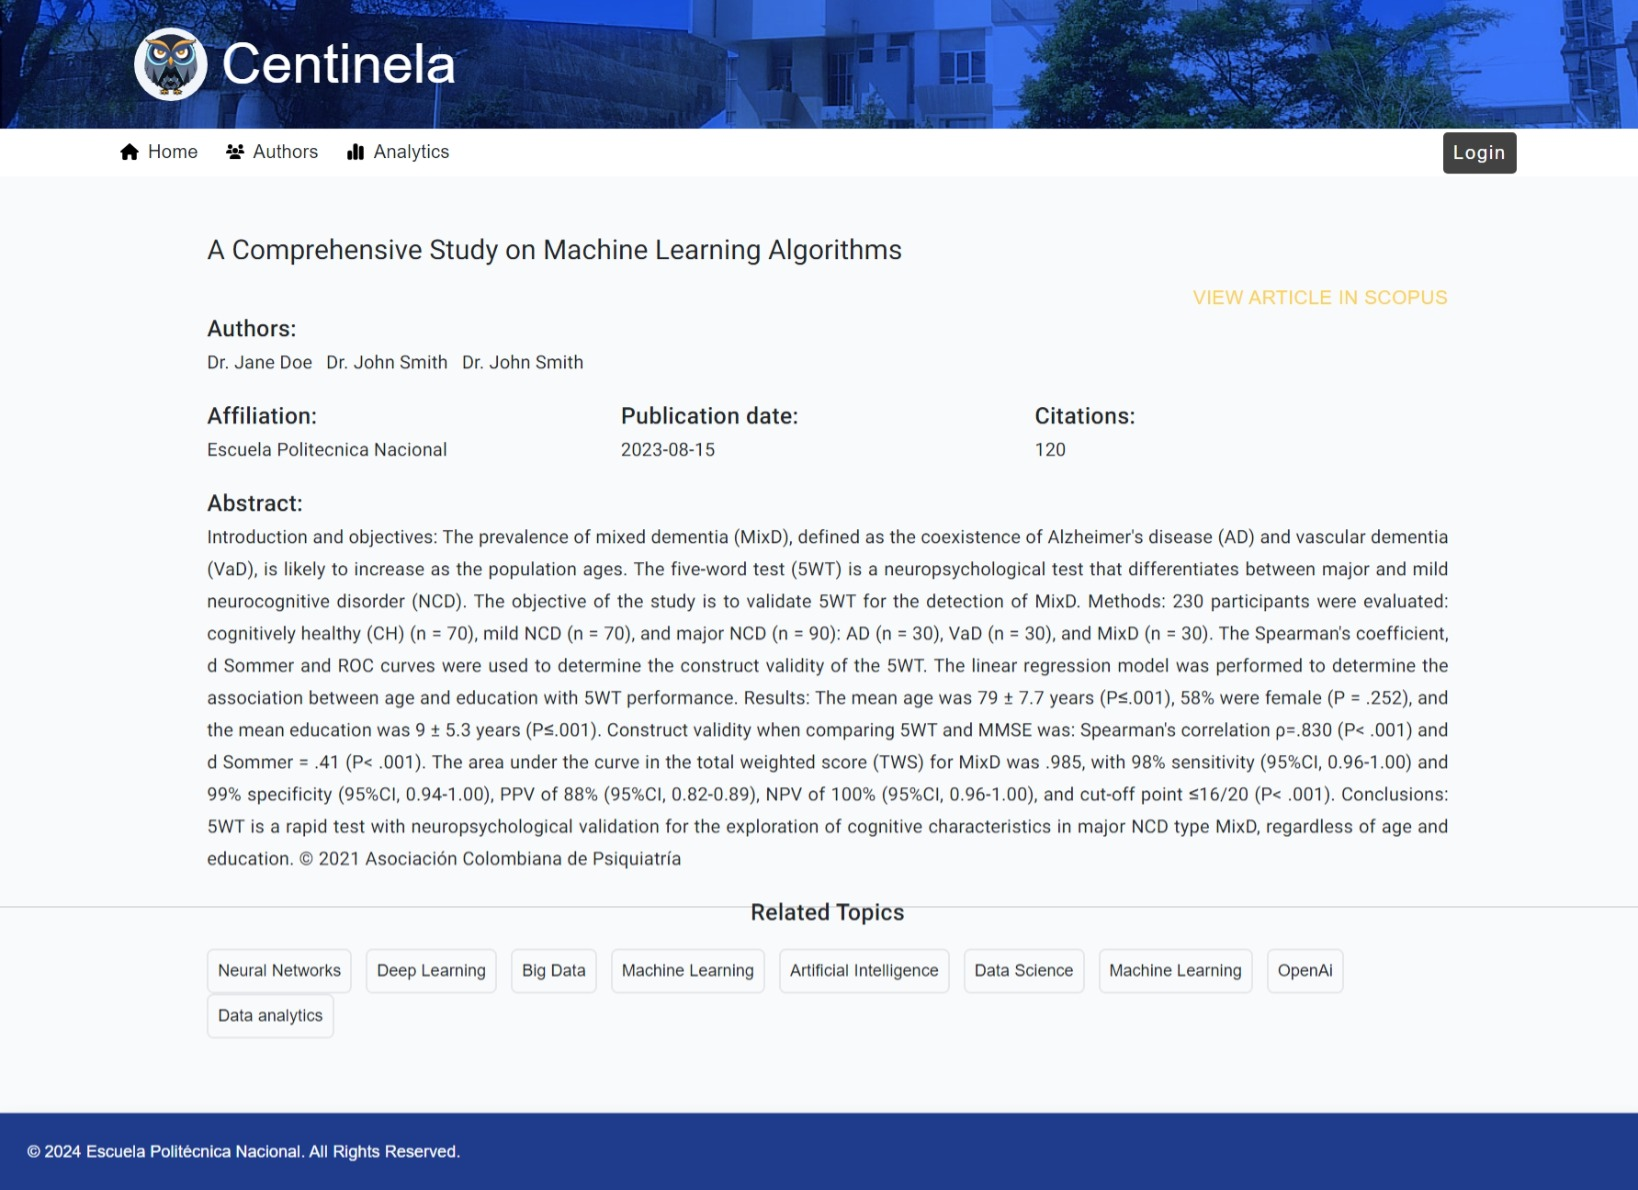
\includegraphics[scale=0.160]{../02Figures/02Chapter/Sprints/Sprint-1/article-page.jpeg}
    \caption{Página de detalle de articulo}
    \label{fig:article-page}
\end{figure}

%% Revision y Retrospectiva del sprint
\subsection{Revisión y Retrospectiva}
Durante este sprint, hemos logrado completar todas las historias de usuario planificadas, lo que nos ha permitido avanzar significativamente en el desarrollo de la aplicación.
Hemos creado los mockups de las interfaces de usuario de la aplicación, desarrollado la estructura principal del motor de búsqueda, implementado el enrutamiento de la aplicación y la página de inicio.
Además, hemos implementado la página de resultados y la página de información general de un artículo.
En general, el equipo ha trabajado de manera eficiente y colaborativa, lo que ha permitido cumplir con los objetivos del sprint en el tiempo previsto.
Sin embargo, hemos identificado algunas áreas de mejora que podrían ayudarnos a optimizar nuestro trabajo en futuros sprints.
\begin{itemize}
    \item \textbf{Comunicación}: Aunque hemos mantenido una comunicación constante a través de reuniones diarias y canales de mensajería, es importante mejorar la comunicación entre los miembros del equipo para garantizar que todos estén al tanto de los avances del proyecto.
    \item \textbf{Planificación}: Aunque hemos logrado completar todas las historias de usuario planificadas, es importante revisar y ajustar nuestra planificación para futuros sprints, teniendo en cuenta la complejidad y el tiempo requerido para cada tarea.
    \item \textbf{Colaboración}: Hemos trabajado de manera colaborativa y eficiente durante este sprint, lo que ha permitido cumplir con los objetivos del proyecto. Es importante seguir fomentando la colaboración entre los miembros del equipo para garantizar el éxito del proyecto.
    \item \textbf{Retroalimentación}: Es importante recopilar y analizar la retroalimentación de los usuarios para identificar áreas de mejora y realizar ajustes en futuras iteraciones del proyecto.
\end{itemize}

Cabe destacar que las tareas referentes a la integración de la aplicación con la API de Scopus, así como la implementación de funcionalidades del lado del servidor,
se han dejado para futuros sprints, ya que requieren un mayor tiempo de desarrollo y dependen de la finalización de otras tareas.